\subsection{bpmsimulation/bpm\_\-simulation.h File Reference}
\label{bpm__simulation_8h}\index{bpmsimulation/bpm\_\-simulation.h@{bpmsimulation/bpm\_\-simulation.h}}


\subsubsection{Detailed Description}
libbpm waveform simulation routines 

This header contains the definitions for the libbpm RF waveform simulation routines 

Definition in file {\bf bpm\_\-simulation.h}.

{\tt \#include $<$math.h$>$}\par
{\tt \#include $<$bpm/bpm\_\-defs.h$>$}\par
{\tt \#include $<$bpm/bpm\_\-interface.h$>$}\par
{\tt \#include $<$bpm/bpm\_\-wf.h$>$}\par
{\tt \#include $<$bpm/bpm\_\-nr.h$>$}\par
{\tt \#include $<$bpm/bpm\_\-dsp.h$>$}\par


Include dependency graph for bpm\_\-simulation.h:\nopagebreak
\begin{figure}[H]
\begin{center}
\leavevmode
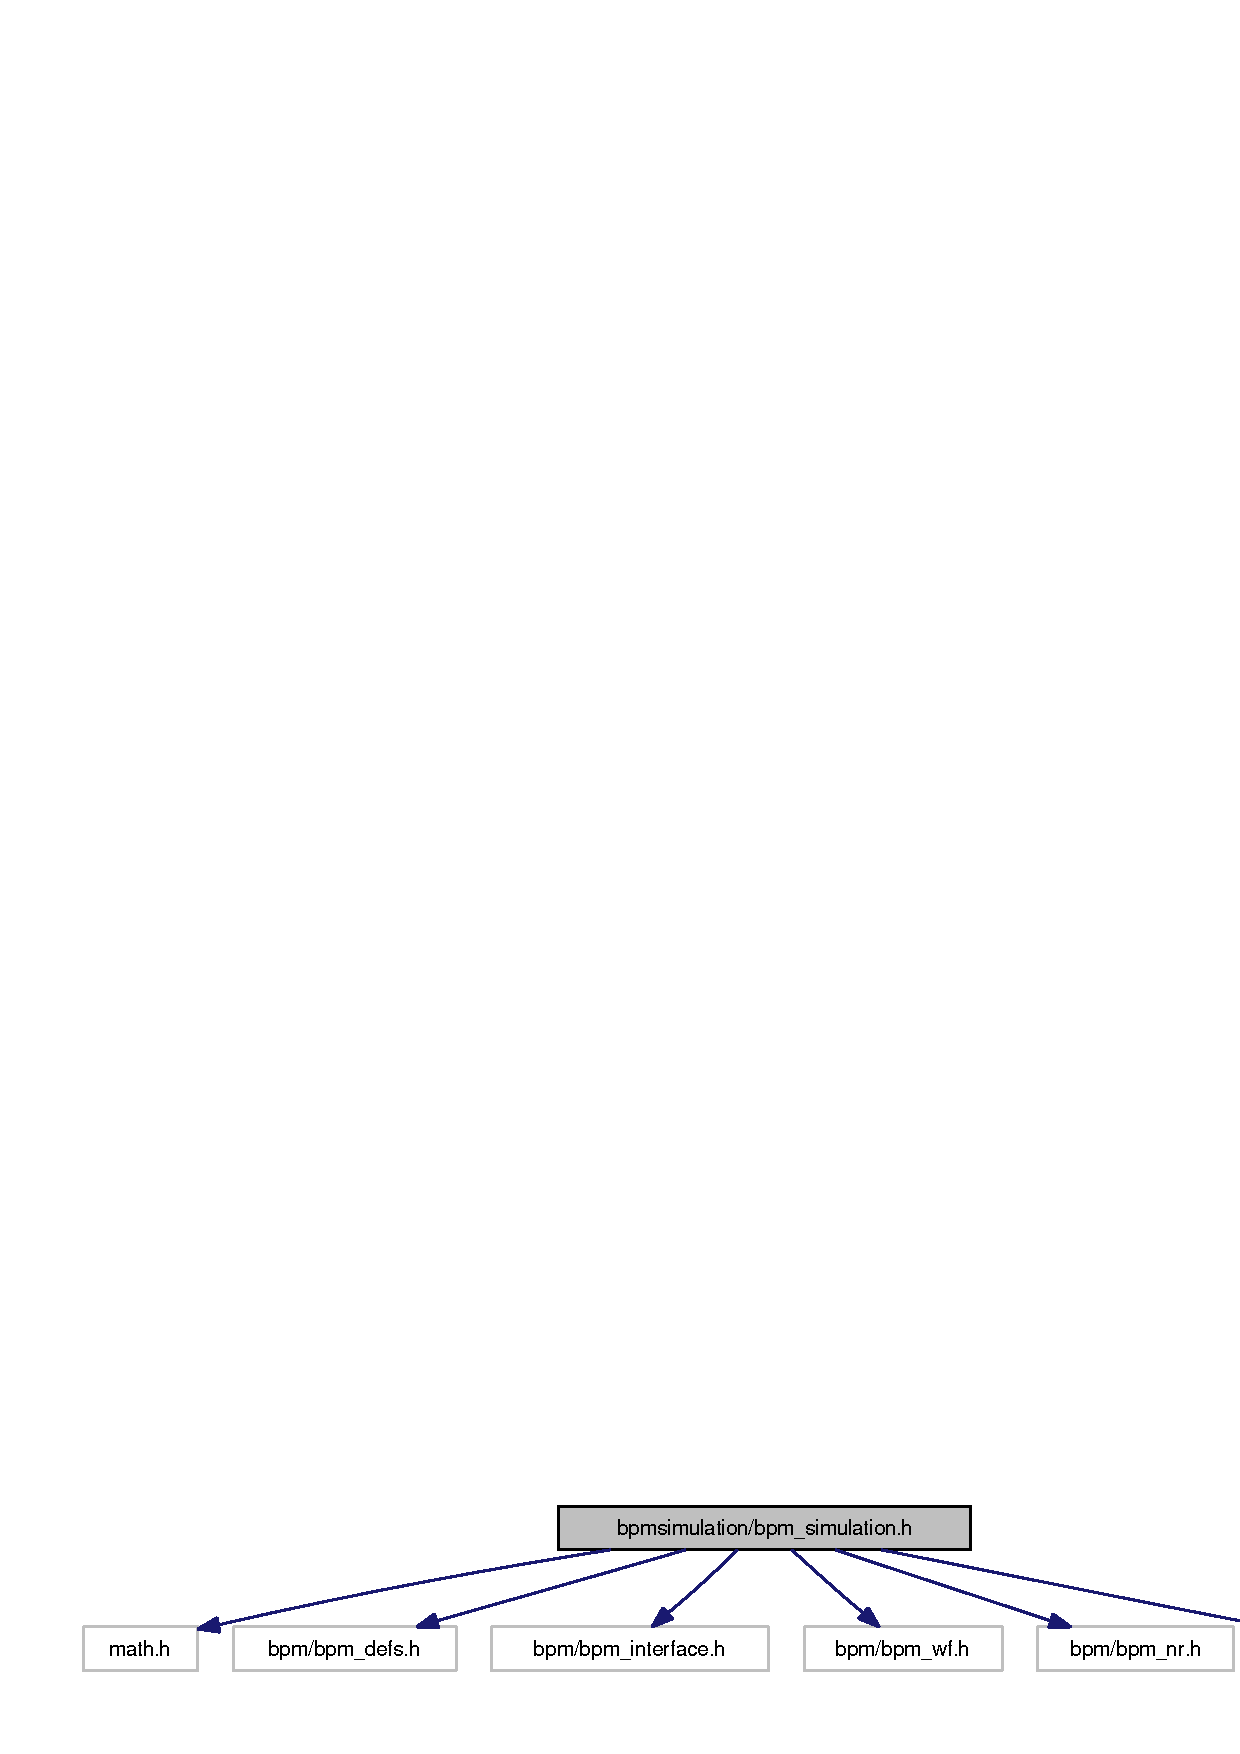
\includegraphics[width=358pt]{bpm__simulation_8h__incl}
\end{center}
\end{figure}
\subsubsection*{Defines}
\begin{CompactItemize}
\item 
\#define {\bf K\_\-SAMPLE}
\item 
\#define \textbf{MODE\_\-DECAY}\label{group__sim_g057113600a8f0d237093da56f7c6b490}

\item 
\#define \textbf{MODE\_\-MAX\_\-SAMPLES}\label{group__sim_g26762c236ebdbdf60197a9aa519bf6aa}

\end{CompactItemize}
\subsubsection*{Functions}
\begin{CompactItemize}
\item 
EXTERN int {\bf set\_\-temp} (double TK)
\item 
EXTERN int {\bf set\_\-time} (double ts)
\item 
EXTERN int {\bf generate\_\-bpmsignal} ({\bf bpmconf\_\-t} $\ast$bpm, {\bf bpmmode\_\-t} $\ast$mode, {\bf beamconf\_\-t} $\ast$beam, {\bf doublewf\_\-t} $\ast$rf)
\item 
EXTERN int {\bf add\_\-mode\_\-response} ({\bf bpmconf\_\-t} $\ast$bpm, {\bf bpmmode\_\-t} $\ast$mode, {\bf bunchconf\_\-t} $\ast$bunch, {\bf doublewf\_\-t} $\ast$rf)
\item 
EXTERN {\bf complex\_\-t} {\bf get\_\-mode\_\-amplitude} ({\bf bpmconf\_\-t} $\ast$bpm, {\bf bpmmode\_\-t} $\ast$mode, {\bf bunchconf\_\-t} $\ast$bunch)
\item 
EXTERN {\bf doublewf\_\-t} $\ast$ {\bf generate\_\-diodesignal} ({\bf doublewf\_\-t} $\ast$rf, double sens, {\bf filter\_\-t} $\ast$filt, triggertype\_\-t diode)
\item 
EXTERN int {\bf get\_\-mode\_\-response} ({\bf bpmmode\_\-t} $\ast$mode)
\item 
EXTERN int {\bf digitise} ({\bf doublewf\_\-t} $\ast$IF, int nbits, double range\_\-min, double range\_\-max, double clock\_\-jitter, double digi\_\-noise, unsigned int ipmode, {\bf intwf\_\-t} $\ast$wf)
\end{CompactItemize}
\subsubsection*{Variables}
\begin{CompactItemize}
\item 
EXTERN double {\bf ambient\_\-temp}
\item 
EXTERN double {\bf system\_\-time}
\end{CompactItemize}
